%! Author = breandan
%! Date = 2/22/24

% Preamble
\documentclass[11pt]{article}

% Packages
\usepackage{amsmath}

\usepackage{tikz}
\usepackage{amssymb}
\usetikzlibrary{shapes.geometric, arrows}

\tikzstyle{startstop} = [rectangle, rounded corners,
minimum width=3cm,
minimum height=1cm,
thick,
text centered,
draw=black,
fill=red!30]

\tikzstyle{io} = [trapezium,
trapezium stretches=true, % A later addition
thick,
trapezium left angle=70,
trapezium right angle=110,
minimum width=3cm,
minimum height=1cm, text centered,
draw=black, fill=blue!30]

\tikzstyle{process} = [rectangle,
minimum width=3.5cm,
minimum height=1cm,
thick,
text centered,
text width=4cm,
draw=black,
fill=orange!30]

\tikzstyle{decision} = [diamond,
minimum width=3cm,
minimum height=1cm,
thick,
text centered,
draw=black,
fill=green!30]
\tikzstyle{arrow} = [->,thick]
\begin{document}

% Document
\begin{document}

\section{Method}

The syntax of most programming languages is context-free. Our proposed method is simple. We construct a context-free grammar representing the intersection between the langauge syntax and an automaton recognizing the Levenshtein ball of a given radius. Since CFLs are closed under intersection with regular languages, this is admissible. Three outcomes are possible:

\begin{enumerate}
  \item $\mathcal{G}_\cap$ is empty, in which case there is no repair within the given radius. In this case, we simply increase the radius and try again.
  \item $\mathcal{L}(\mathcal{G}_\cap)$ is small, in which case we simply enumerate all possible repairs. Enumeration is tractable for $\sim 80\%$ of the Python dataset in $\leq 90$s.
  \item $\mathcal{L}(\mathcal{G}_\cap)$ is too large to enumerate, so we sample from the intersection grammar $\mathcal{G}_\cap$. Sampling is necessary for $\sim20\%$ of the Python dataset.
\end{enumerate}

When ambiguous, we use an n-gram model to rank and return the top-k results by likelihood. This procedure is depicted in the flowchart below:

\begin{figure}[h!]
  \begin{center}
\resizebox{0.6\textwidth}{!}{
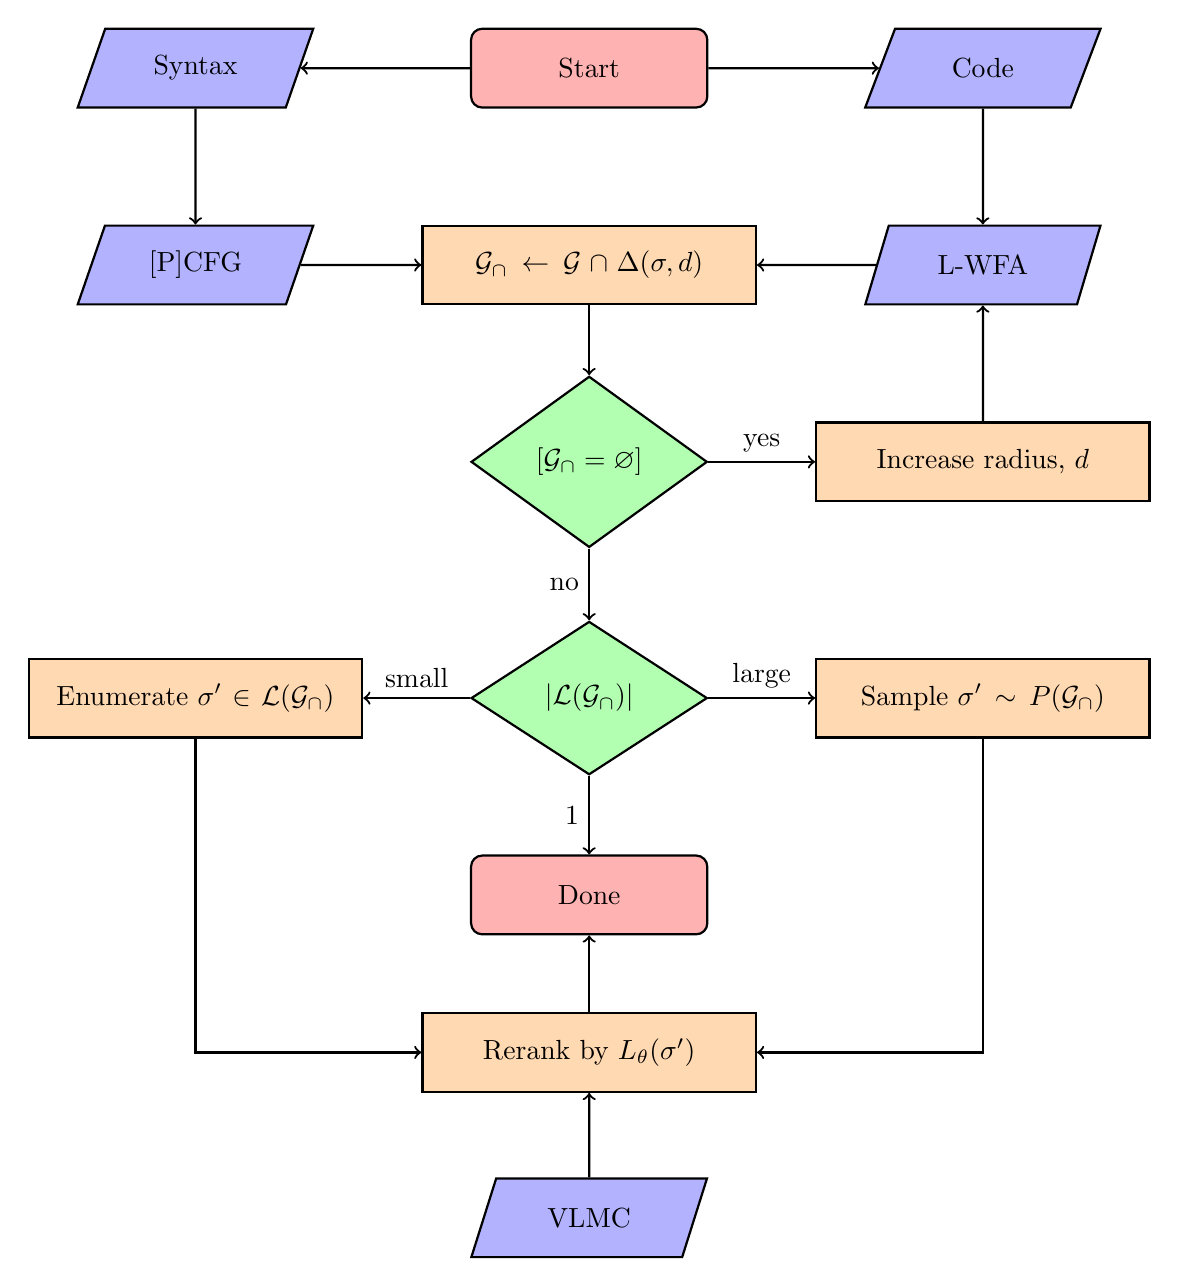
\begin{tikzpicture}[node distance=2cm]

  \node (start) [startstop] {Start};
  \node (pro1) [process, below of=start, yshift=-0.5cm] {$\mathcal{G}_\cap \leftarrow \mathcal{G}\cap\Delta(\err\sigma, d)$};
  \node (pcfg) [io, left of=pro1, xshift=-3cm] {[P]CFG};
  \node (lnfa) [io, right of=pro1, xshift=3cm] {L-WFA};

  \node (code) [io, right of=start,xshift=3cm] {Code};
  \node (synt) [io, left of=start,xshift=-3cm] {Syntax};

  \node (dec1) [decision, below of=pro1, yshift=-0.5cm] {$[\mathcal{G}_{\cap} = \varnothing]$};

  \node (pro2b) [process, right of=dec1, xshift=3cm] {Increase radius, $d$};

  \node (dec2) [decision, below of=dec1, yshift=-1cm] {$|\mathcal{L}(\mathcal{G}_\cap)|$};

  \node (samp1) [process, left of=dec2, xshift=-3cm] {Enumerate $\sigma' \in \mathcal{L}(\mathcal{G}_\cap)$};
  \node (samp2) [process, right of=dec2, xshift=3cm] {Sample $\sigma' \sim P(\mathcal{G}_\cap)$};

  \node (rank) [process, below of=dec2, yshift=-2.5cm] {Rerank by $L_\theta(\sigma')$};
  \node (vlmc) [io, below of=rank, yshift=-0.1cm] {VLMC};

%  \node (out1) [io, below of=pro2a] {Output};
  \node (stop) [startstop, above of=rank] {Done};

%  \draw [arrow] (dec0) -- node[anchor=east] {no} (pro1);

  \draw [arrow] (start) -- (code);
  \draw [arrow] (start) -- (synt);
  \draw [arrow] (code) -- (lnfa);
  \draw [arrow] (synt) -- (pcfg);
  \draw [arrow] (lnfa) -- (pro1);
  \draw [arrow] (pcfg) -- (pro1);

%  \draw [arrow] (in1) -- (pro1);
  \draw [arrow] (pro1) -- (dec1);
  \draw [arrow] (dec1) -- node[anchor=south] {yes} (pro2b);
  \draw [arrow] (dec1) -- node[anchor=east] {no} (dec2);
  \draw [arrow] (pro2b) -- (lnfa);
  \draw [arrow] (dec2) -- node[anchor=south] {small} (samp1);
  \draw [arrow] (dec2) -- node[anchor=south] {large} (samp2);

  \draw [arrow] (vlmc) -- (rank);
  \draw [arrow] (samp1) |- (rank);
  \draw [arrow] (samp2) |- (rank);
%  \draw [arrow] (pro2a) -- (out1);
  \draw [arrow] (rank) -- (stop);
  \draw [arrow] (dec2) -- node[anchor=east] {1} (stop);

\end{tikzpicture}
}
\end{center}
\caption{Flowchart of our proposed method.}\label{fig:flowchart}
\end{figure}

\subsection{The Nominal Levenshtein Automaton}

Levenshtein edits are recognized by a certain kind of automaton, known as the Levenshtein automaton. Since the original approach used by Schultz and Mihov contains cycles and epsilon transitions, we propose a modified variant which is epsilon-free, acyclic and monotone. Furthermore, we use a nominal automaton, allowing for infinite alphabets. This considerably simplifies the langauge intersection.

\subsection{The Bar-Hillel Construction}

The Bar-Hillel construction is a general method for obtaining the context-free grammar representing the intersection of a context-free language and a regular language. We will now present the epsilon-free version of the Bar-Hillel construction used in our work.\footnote{Clemente Pasti has a version of the BH construction that supports epsilon transitions, but is slightly more complicated.}

\subsection{The Levenshtein-Bar-Hillel-Parikh Reduction}

The standard BH construction applies to any CFL and REG language. While straightforward, the general method can generate hundreds of trillions of productions for moderately sized grammars and Levenshtein automata. Our method considerably simplifies this process by eliminating the need to materialize most of those productions, and is the key to making our approach tractable.

To achieve this, we precompute upper and lower Parikh bounds for every terminal and integer range of the string, which we call the Parikh map. This construction soundly overapproximates the minimum and maximum number of terminals that can be derived from a given nonterminal in a bounded-length string, and is used to prune the search space. We will now describe this reduction in detail.



\end{document}